\documentclass[conference]{IEEEtran}
\IEEEoverridecommandlockouts

\usepackage{cite}
\usepackage{amsmath,amssymb,amsfonts}
\usepackage{algorithmic}
\usepackage{algorithm}
\usepackage{graphicx}
\usepackage{textcomp}
\usepackage{xcolor}
\usepackage{booktabs}
\usepackage{multirow}
\usepackage{url}
\usepackage{tikz}
\usetikzlibrary{shapes.geometric, arrows.meta, positioning, fit, calc, backgrounds}
\def\BibTeX{{\rm B\kern-.05em{\sc i\kern-.025em b}\kern-.08em
    T\kern-.1667em\lower.7ex\hbox{E}\kern-.125emX}}

\begin{document}

\title{Mengatasi Ketidakseimbangan Kelas Ekstrem dalam Segmentasi Kebakaran Hutan: Pendekatan Gabungan Loss dan Berpusat pada Data\\}

\author{\IEEEauthorblockN{1\textsuperscript{st} Author Name}
\IEEEauthorblockA{\textit{dept. name of organization (of Aff.)} \\
\textit{name of organization (of Aff.)}\\
City, Country \\
email address or ORCID}
\and
\IEEEauthorblockN{2\textsuperscript{nd} Author Name}
\IEEEauthorblockA{\textit{dept. name of organization (of Aff.)} \\
\textit{name of organization (of Aff.)}\\
City, Country \\
email address or ORCID}
\and
\IEEEauthorblockN{3\textsuperscript{rd} Author Name}
\IEEEauthorblockA{\textit{dept. name of organization (of Aff.)} \\
\textit{name of organization (of Aff.)}\\
City, Country \\
email address or ORCID}
\and
\IEEEauthorblockN{4\textsuperscript{th} Author Name}
\IEEEauthorblockA{\textit{dept. name of organization (of Aff.)} \\
\textit{name of organization (of Aff.)}\\
City, Country \\
email address or ORCID}
\and
\IEEEauthorblockN{5\textsuperscript{th} Author Name}
\IEEEauthorblockA{\textit{dept. name of organization (of Aff.)} \\
\textit{name of organization (of Aff.)}\\
City, Country \\
email address or ORCID}
\and
\IEEEauthorblockN{6\textsuperscript{th} Author Name}
\IEEEauthorblockA{\textit{dept. name of organization (of Aff.)} \\
\textit{name of organization (of Aff.)}\\
City, Country \\
email address or ORCID}
}

\maketitle

\begin{abstract}
Deteksi otomatis kebakaran dan asap melalui jaringan kamera jarak jauh sangat penting untuk memitigasi dampak kebakaran hutan. Meskipun model segmentasi semantik menawarkan batas tingkat piksel yang presisi, penerapannya sangat terhambat oleh ketidakseimbangan dataset yang ekstrem. Pada citra kebakaran hutan, objek target menempati sebagian kecil dari bingkai beresolusi tinggi, dan terdapat ketidakseimbangan intrakelas yang drastis di mana asap difus jauh lebih banyak daripada bagian depan api aktif. Dalam makalah ini, kami menunjukkan secara empiris bahwa pipeline segmentasi naif gagal secara bencana pada kelas api minoritas, hanya mencapai 62,1\% Fire mIoU pada dataset FIgLib. Untuk mengatasi hal ini, kami mengusulkan pipeline optimasi yang berpusat pada formulasi Combined Loss (Lovasz-Softmax, Focal, dan Dice) khusus yang secara eksplisit menyelamatkan kelas minoritas, meningkatkan Fire mIoU menjadi 79,9\%. Selanjutnya, kami memperkenalkan optimasi berpusat pada data sekunder---yaitu transformasi ruang warna RGCr dan algoritme Balanced SAHI-style Tiling---yang memaksa jaringan untuk memprioritaskan tanda termal api aktif dibandingkan asap difus. Studi ablasional kami mengungkap pertukaran penting: sementara Combined Loss saja menghasilkan akurasi keseluruhan tertinggi (79,9\% Fire+Smoke mIoU), penambahan strategi RGCr dan Tiling kami berhasil mendorong Fire mIoU ke state-of-the-art 81,1\%, mengorbankan sebagian kecil presisi batas asap untuk menjamin deteksi peristiwa pembakaran kritis.
\end{abstract}

\begin{IEEEkeywords}
Segmentasi Semantik, Deteksi Kebakaran Hutan, Ketidakseimbangan Kelas, Combined Loss, PIDNet, Ruang Warna, Tiling
\end{IEEEkeywords}

\section{Pendahuluan}
Proliferasi sistem pengawasan jarak jauh berbasis kamera yang cepat telah memposisikan visi komputer sebagai teknologi pelopor untuk deteksi dini kebakaran hutan. Tidak seperti kotak pembatas deteksi objek yang mendasar, segmentasi semantik mengklasifikasikan gambar pada tingkat piksel, memberikan batas morfologis yang presisi. Akurasi tingkat piksel ini sangat penting bagi sistem manajemen bencana di hilir, karena memungkinkan ekstraksi parameter fisik vital—seperti volume api, vektor perambatan, dan laju penyebaran—yang penting untuk mengerahkan penanggap pertama secara efektif.

Namun, penerapan model segmentasi di alam liar memperkenalkan masalah yang sangat parah dan sering melemahkan yang berpusat pada data. Masalah mendasarnya adalah ketidakseimbangan kelas yang ekstrem, yang terwujud dalam dua cara berbeda. Pertama, terdapat ketidakseimbangan latar depan-latar belakang yang drastis. Pada citra kamera jarak jauh beresolusi tinggi, objek yang menjadi perhatian (api dan asap) menempati sebagian kecil dari total ruang piksel dibandingkan dengan latar belakang yang luas (misalnya, langit, dedaunan, pegunungan). Kedua, dan yang lebih kritis, terdapat ketidakseimbangan intrakelas yang parah: asap difus jauh lebih umum, besar, dan terlihat daripada bagian depan api aktif itu sendiri. Dalam subset dataset FIgLib (Fire Image Library) yang kami analisis, disparitas intrakelas ini terwujud sebagai rasio anotasi Api-terhadap-Asap yang mengejutkan sebesar 1:7.

Ketika metodologi pelatihan standar dan fungsi loss (seperti Cross-Entropy) diterapkan pada dataset yang tidak seimbang tersebut, model deep learning selalu jatuh ke dalam jebakan statistik. Model dengan cepat belajar meminimalkan loss global dengan menjadi sangat mahir dalam mengklasifikasikan kelas mayoritas (latar belakang dan asap) sambil mengabaikan kelas minoritas secara fungsional (api aktif). Hal ini menghasilkan model yang membanggakan akurasi keseluruhan yang tinggi tetapi secara fungsional tidak berguna untuk tugas utamanya: mendeteksi api yang sebenarnya. Lebih jauh lagi, praktik pemuatan data standar memperburuk masalah ini. Citra pengawasan resolusi tinggi biasanya diturunkan sampelnya (downsampled) agar sesuai dengan kendala memori GPU, sebuah proses yang secara permanen menghancurkan fitur spasial frekuensi tinggi dari bagian depan api mikroskopis tahap awal.

Dalam makalah ini, kami mengusulkan metodologi yang komprehensif dan didorong oleh masalah untuk memecahkan ketidakseimbangan kelas dan tantangan resolusi ini. Dengan memanfaatkan Proportional-Integral-Derivative Network (PIDNet) \cite{pidnet} yang sangat efisien sebagai arsitektur dasar kami, hasil empiris kami menunjukkan bahwa pilihan arsitektural saja tidak cukup. Sebaliknya, kami mengusulkan pipeline data dan loss yang sangat dioptimalkan.

Kontribusi utama makalah ini adalah:
\begin{itemize}
    \item Kami menunjukkan bahwa strategi Combined Loss khusus (mensinergikan Lovasz-Softmax, Focal Loss, dan Dice Loss dengan pembobotan kelas yang agresif) merupakan intervensi tunggal yang paling efektif untuk ketidakseimbangan ekstrem, secara mandiri meningkatkan Fire mIoU dari 62,1\% menjadi 79,9\%.
    \item Kami memperkenalkan transformasi ruang warna RGCr (Red, Green, Chrominance-Red) dan algoritme Balanced Tiling deterministik untuk memerangi hilangnya resolusi dan memprioritaskan tanda termal api aktif di atas asap difus.
    \item Kami menyajikan studi ablasional yang komprehensif pada dataset FIgLib, memberikan wawasan yang dapat ditindaklanjuti ke dalam pertukaran presisi-recall yang diperlukan untuk sistem pemantauan bencana yang kritis terhadap kehidupan.
\end{itemize}

\section{Pekerjaan Terkait}

\subsection{Deteksi dan Segmentasi Kebakaran Hutan}
Deteksi visual dini kebakaran hutan mengandalkan ambang batas buatan tangan untuk warna dan tekstur, yang sangat rentan terhadap false positive dari awan dan silau matahari. Meskipun peralihan ke deep learning secara signifikan meningkatkan generalisasi, model modern masih sangat kesulitan dengan false positive yang disebabkan oleh awan dataran rendah, kabut, dan kabut atmosfer \cite{govil2020preliminary, nguyen2023smokeynet}. Lebih jauh lagi, persyaratan pemrosesan pada kamera jarak jauh telah mendorong adopsi arsitektur yang sangat efisien seperti BiSeNet dan PIDNet, yang menyeimbangkan resolusi spasial dengan kecepatan inferensi yang cepat. Namun, jaringan ringan ini sangat rentan terhadap ketidakseimbangan kelas yang ekstrem dan "masalah objek kecil"---di mana kebakaran tahap awal hanya menempati segelintir piksel---karena mereka kekurangan jumlah parameter masif yang diperlukan untuk menghafal distribusi kelas minoritas yang kompleks.

\subsection{Mengatasi Ketidakseimbangan Kelas}
Ketidakseimbangan kelas adalah masalah yang meresap dalam visi komputer. Pada tingkat data, teknik seperti oversampling atau SMOTE umum digunakan, meskipun sulit diterapkan pada mask segmentasi padat. Pada tingkat algoritme, fungsi loss khusus telah terbukti sangat efektif. Focal Loss \cite{focal} memodifikasi Cross-Entropy untuk secara dinamis menurunkan bobot contoh latar belakang "mudah". Lovasz-Softmax loss \cite{lovasz} memberikan pengganti yang mulus dan dapat didiferensialkan untuk Jaccard index (IoU) diskrit, memungkinkan jaringan untuk mengoptimalkan tumpang tindih set secara langsung tanpa memandang frekuensi kelas.

\subsection{Menangani Objek Kecil dan Ruang Warna}
Untuk mengatasi "masalah objek kecil" yang disebabkan oleh downsampling citra resolusi tinggi, Slicing Aided Hyper Inference (SAHI) \cite{sahi} sering digunakan untuk menyimpulkan pada patch tumpang tindih resolusi tinggi. Selain itu, para peneliti telah menemukan keberhasilan memanipulasi ruang warna (misalnya, YCbCr, atau HSV \cite{muhammad2023fire}) untuk mengisolasi tanda pencahayaan (luminance) dan krominansi (chrominance) pembakaran, mencegah jaringan membingungkan asap putih dengan awan.

\subsection{Arsitektur Segmentasi Dasar (PIDNet)}
Berbeda dengan arsitektur segmentasi konvensional yang sering kali mengorbankan detail batas demi konteks semantik, PIDNet \cite{pidnet} diperkenalkan untuk memberikan keseimbangan yang optimal. Terinspirasi dari pengontrol Proportional-Integral-Derivative (PID), jaringan ini menggunakan arsitektur tiga cabang (\textit{three-branch}) yang dirancang untuk secara bersamaan memproses detail spasial (Proportional), konteks semantik tingkat tinggi (Integral), dan batas atau batas objek (Derivative). Desain tiga cabang ini membuatnya secara unik cocok untuk mempertahankan batas-batas tajam mikroskopis dari kebakaran tahap awal---sebuah area di mana jaringan encoder-decoder seperti UNet secara tradisional kesulitan---sambil mempertahankan efisiensi tinggi untuk memproses gambar beresolusi tinggi. Namun, seperti yang akan ditunjukkan dalam makalah ini, meskipun PIDNet secara inheren kuat dalam menjaga detail batas, arsitektur ini tetap membutuhkan penyesuaian khusus pada level data dan fungsi \textit{loss} ketika dihadapkan pada ketidakseimbangan kelas yang ekstrem.

\subsection{Sumber Data}
Sebagian besar penelitian awal mengenai deteksi kebakaran bergantung pada kumpulan data skala kecil atau gambar tak beraturan yang dikumpulkan dari internet. Seiring berkembangnya pendekatan \textit{deep learning}, beberapa basis data khusus mulai tersedia, seperti Corsican Fire Database dan dataset FLAME yang menyediakan data video maupun citra termal. Namun, untuk pelatihan model segmentasi semantik yang membutuhkan anotasi batas tingkat piksel yang sangat presisi pada kondisi lingkungan liar, FIgLib (Fire Image Library) yang disediakan oleh HPWREN menjadi salah satu sumber data yang paling komprehensif. Dataset ini mencakup citra beresolusi tinggi dari kamera jarak jauh dalam kondisi nyata, yang meskipun sangat berharga, membawa tantangan tersendiri berupa ketidakseimbangan kelas yang ekstrem antara asap, api, dan latar belakang.

\section{Metodologi}
\label{sec:methodology}

Metodologi yang kami usulkan mengatasi kegagalan pipeline segmentasi naif melalui pendekatan dua cabang: strategi Combined Loss khusus untuk memerangi ketidakseimbangan kelas pada tingkat gradien, dan serangkaian optimasi berpusat pada data (Temporal Pruning, Color Space Transformation, dan Balanced Tiling) yang dirancang untuk memprioritaskan tanda termal dari bagian depan api di atas asap difus.

\begin{figure}[htbp]
\centering
\resizebox{\columnwidth}{!}{%
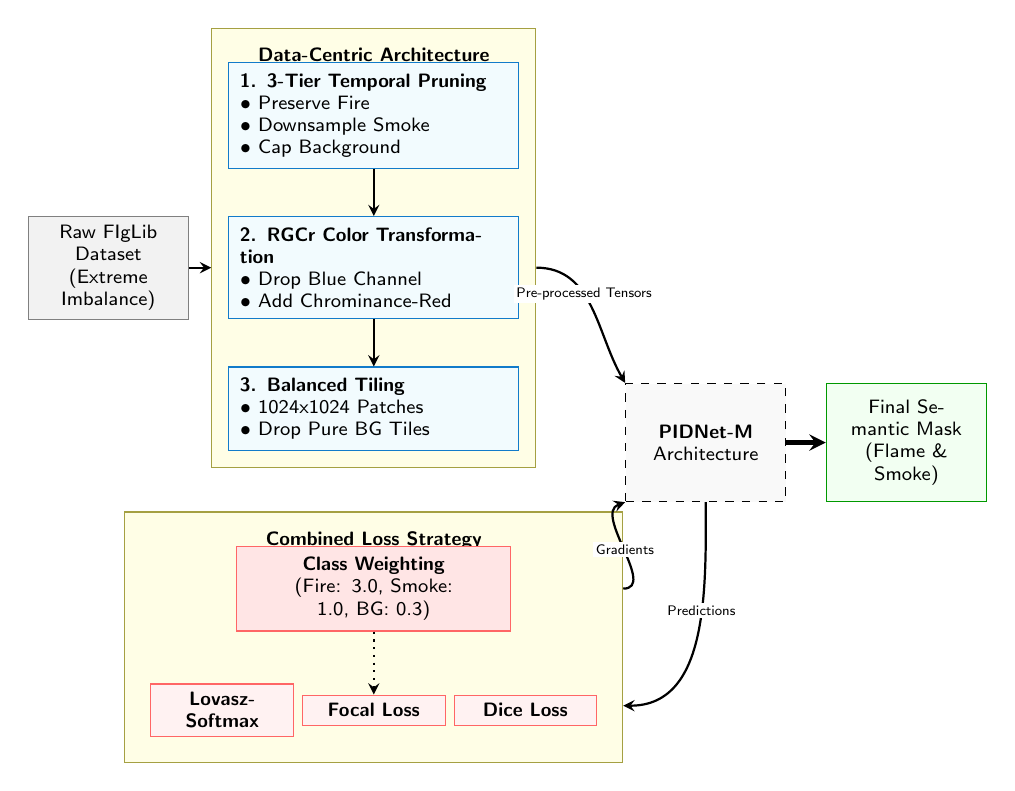
\begin{tikzpicture}[
    node distance=0.6cm and 0.5cm,
    font=\sffamily\scriptsize,
    >=stealth,
    % Styles
    raw/.style={rectangle, draw=gray, fill=gray!10, text width=1.8cm, align=center, minimum height=1.2cm},
    datablock/.style={rectangle, draw=cyan!60!blue, fill=cyan!5, text width=3.4cm, align=left, inner sep=4pt},
    lossblock/.style={rectangle, draw=red!60, fill=red!5, text width=1.6cm, align=center, inner sep=3pt},
    classweight/.style={rectangle, draw=red!60, fill=red!10, text width=3.2cm, align=center, inner sep=4pt},
    pidnet/.style={rectangle, draw=black, dashed, fill=gray!5, text width=1.8cm, align=center, minimum height=1.5cm},
    mask/.style={rectangle, draw=green!60!black, fill=green!5, text width=1.8cm, align=center, minimum height=1.5cm},
    grouplabel/.style={font=\sffamily\bfseries\scriptsize, anchor=north},
    groupbox/.style={rectangle, draw=yellow!60!black, fill=yellow!10, inner sep=6pt},
    arrowtext/.style={fill=white, inner sep=1pt, font=\sffamily\tiny}
]

% --- Data Centric Group (Top) ---
\node[datablock] (pruning) {
    \textbf{1. 3-Tier Temporal Pruning}\\
    $\bullet$ Preserve Fire\\
    $\bullet$ Downsample Smoke\\
    $\bullet$ Cap Background
};
\node[datablock, below=of pruning] (rgcr) {
    \textbf{2. RGCr Color Transformation}\\
    $\bullet$ Drop Blue Channel\\
    $\bullet$ Add Chrominance-Red
};
\node[datablock, below=of rgcr] (tiling) {
    \textbf{3. Balanced Tiling}\\
    $\bullet$ 1024x1024 Patches\\
    $\bullet$ Drop Pure BG Tiles
};

% Draw arrows between data blocks
\draw[->, thick] (pruning) -- (rgcr);
\draw[->, thick] (rgcr) -- (tiling);

% Create Data Centric Background Box
\begin{scope}[on background layer]
    \node[groupbox, fit=(pruning) (rgcr) (tiling)] (databg) {};
    \node[groupbox, fit=(pruning) (rgcr) (tiling) (databg.north)] (databg) {};
    \node[grouplabel, yshift=-4pt] at (databg.north) {Data-Centric Architecture};
\end{scope}

% --- Raw Data ---
\node[raw, left=0.5cm of rgcr] (rawdata) {Raw FIgLib Dataset\\(Extreme Imbalance)};
\draw[->, thick] (rawdata) -- (databg.west |- rgcr);

% --- Combined Loss Group (Bottom) ---
\node[classweight, below=1.2cm of tiling] (weights) {
    \textbf{Class Weighting}\\
    (Fire: 3.0, Smoke: 1.0, BG: 0.3)
};

\node[lossblock, below=0.8cm of weights] (focal) {\textbf{Focal Loss}};
\node[lossblock, left=0.1cm of focal] (lovasz) {\textbf{Lovasz-Softmax}};
\node[lossblock, right=0.1cm of focal] (dice) {\textbf{Dice Loss}};

% Draw dotted arrow for weights
\draw[->, thick, dotted] (weights) -- (focal);

% Create Loss Component Box inside Loss Group
\begin{scope}[on background layer]
    \node[rectangle, draw=olive, inner sep=3pt, fit=(lovasz) (focal) (dice)] (losscomp) {};
    \node[rectangle, draw=olive, inner sep=3pt, fit=(lovasz) (focal) (dice) (losscomp.north)] (losscomp) {};
    \node[anchor=south, font=\sffamily\scriptsize, yshift=-5pt] at (losscomp.north) {Loss Components};
    
    % Create Combined Loss Group Box
    \node[groupbox, fit=(weights) (losscomp)] (lossbg) {};
    \node[groupbox, fit=(weights) (losscomp) (lossbg.north)] (lossbg) {};
    \node[grouplabel, yshift=-4pt] at (lossbg.north) {Combined Loss Strategy};
\end{scope}

% --- PIDNet and Mask (Right) ---
\coordinate (middle_right) at ($(databg.east)!0.5!(lossbg.east) + (1.6cm,0)$);
\node[pidnet] (pidnet) at (middle_right) {\textbf{PIDNet-M}\\Architecture};

\node[mask, right=0.5cm of pidnet] (mask) {Final Semantic Mask\\(Flame \& Smoke)};

% --- Connections ---
\draw[->, thick] (databg.east |- rgcr) to[out=0, in=120] node[arrowtext, pos=0.4] {Pre-processed Tensors} (pidnet.north west);
\draw[->, thick] (lossbg.east |- weights) to[out=0, in=200] node[arrowtext, pos=0.5] {Gradients} (pidnet.south west);
\draw[->, thick] (pidnet.south) to[out=270, in=0] node[arrowtext, pos=0.4] {Predictions} (lossbg.east |- losscomp);
\draw[->, ultra thick] (pidnet.east) -- (mask.west);

\end{tikzpicture}
}
\caption{Tinjauan umum tentang arsitektur pipeline yang berpusat pada data yang diusulkan. Rangkaian temporal mentah mengalami pruning 3 tingkat, diikuti oleh isolasi warna RGCr dan Balanced Tiling. Tensor yang dihasilkan diumpankan ke PIDNet-M, dipandu oleh formulasi Combined Loss dengan pembobotan kelas minoritas yang agresif.}
\label{fig:pipeline}
\end{figure}

\subsection{Formulasi Gabungan Loss Ketidakseimbangan}
Kami meninggalkan Cross-Entropy standar dan mendukung Combined Loss $\mathcal{L}_{total}$ yang disesuaikan, yang merupakan penjumlahan tertimbang dari Lovasz-Softmax Loss ($\mathcal{L}_{lovasz}$), Focal Loss ($\mathcal{L}_{focal}$), dan Dice Loss ($\mathcal{L}_{dice}$). 

Pertama, kami mendefinisikan vektor bobot kelas yang agresif dan statis $W_c = [0.3, 3.0, 1.0]$ masing-masing untuk Latar Belakang, Api, dan Asap. Hal ini secara langsung memaksa pengoptimal untuk memperlakukan gradien yang terkait dengan piksel Api 10 kali lebih penting daripada latar belakang.

\textbf{Lovasz-Softmax Loss}: Jaccard index (IoU) adalah metrik evaluasi utama untuk segmentasi, tetapi ini diskrit dan tidak dapat didiferensialkan. Ekstensi Lovasz memberikan pengganti cembung yang mulus. Dengan mengoptimalkan $\mathcal{L}_{lovasz}$, jaringan secara langsung mengoptimalkan metrik tumpang tindih set, yang secara inheren menormalkan terhadap jumlah piksel kelas, memberikan kelegaan besar pada kelas minoritas Api.

\textbf{Focal Loss}: Cross-Entropy standar memberikan kepentingan yang sama untuk semua piksel. Focal loss menurunkan kontribusi piksel latar belakang "mudah" (misalnya, langit biru cerah) yang modelnya sudah dapat mengklasifikasikan dengan percaya diri. Ini memfokuskan pembaruan gradien secara ketat pada piksel batas ambiguitas "sulit" dari asap dan api. Didefinisikan sebagai:
\begin{equation}
    \mathcal{L}_{focal} = - \sum_{c} \alpha_c (1 - p_c)^\gamma \log(p_c)
\end{equation}
Di mana $p_c$ adalah probabilitas yang diprediksi, $\alpha_c$ dipetakan dari bobot kelas kami $W_c$, dan parameter fokus diatur ke $\gamma = 2.0$.

\textbf{Dice Loss}: Serupa dengan Lovasz, Dice loss mengoptimalkan F1-score dari output segmentasi, semakin memperkuat batas. 

Fungsi loss akhir adalah jumlah yang dinormalisasi dari ketiga komponen ini:
\begin{equation}
    \mathcal{L}_{total} = \frac{\lambda_1 \mathcal{L}_{lovasz} + \lambda_2 \mathcal{L}_{focal} + \lambda_3 \mathcal{L}_{dice}}{\lambda_1 + \lambda_2 + \lambda_3}
\end{equation}
Kami menggunakan bobot internal yang seimbang dari $\lambda_1 = 0.33$, $\lambda_2 = 0.33$, dan $\lambda_3 = 0.34$. 

\subsection{Deskripsi Dataset dan Temporal Pruning}
Kami memanfaatkan dataset FIgLib (Fire Image Library), yang terdiri dari urutan temporal gambar yang diambil dari lokasi pemasangan jarak jauh. Dataset mentah tersebut berisi lebih dari $21.383$ gambar khusus latar belakang. Di dalam subset yang dianotasi, terdapat $18.158$ instans asap dibandingkan dengan hanya $1.904$ instans api. Dataset ini dipartisi menjadi set pelatihan (training), validasi (validation), dan pengujian (testing) dengan menggunakan rasio pembagian 80/10/10. 

Untuk memitigasi ketidakseimbangan inter-kelas (Foreground vs. Background) dan intra-kelas (Smoke vs. Fire) yang ekstrem ini, kami mengimplementasikan algoritme temporal pruning 3 tingkat deterministik sebelum dataloading, memanfaatkan prinsip yang mapan dari pengurangan redundansi temporal \cite{wu2019adaframe} dan undersampling kelas mayoritas \cite{drummond2003c4, he2009imbalanced}. Gambar dikelompokkan secara kronologis berdasarkan urutan kejadian. 
\begin{itemize}
    \item \textbf{Tingkat 1 (Pelestarian Api)}: Setiap urutan temporal yang berisi anotasi api aktif dipertahankan secara keseluruhan tanpa downsampling.
    \item \textbf{Tingkat 2 (Downsampling Asap)}: Urutan yang berisi asap tetapi tidak ada api menunjukkan redundansi temporal yang tinggi. Ini diturunkan secara seragam menjadi maksimal 50 frame per urutan.
    \item \textbf{Tingkat 3 (Pembatasan Latar Belakang)}: Urutan latar belakang murni diambil sampelnya secara jarang, dan batasan tetap global sebesar 2.500 gambar latar belakang diberlakukan.
\end{itemize}
Pemangkasan algoritmis ini secara drastis mengurangi redundansi temporal dan secara matematis membatasi rasio sampel positif ke negatif, menggeser distribusi dataset menuju kelas minoritas kritis sebelum menerapkan optimasi loss kami.

\subsection{Transformasi Ruang Warna RGCr}
Saluran RGB standar sangat berkorelasi, dan saluran Biru ($B$) memberikan informasi yang dapat diabaikan mengenai pembakaran. Api memancarkan radiasi terutama di spektrum merah/inframerah. Untuk memanfaatkannya, kami mengusulkan transformasi ruang warna RGCr, membuang saluran Biru dan menggantinya dengan saluran Chrominance-Red ($Cr$) dari ruang warna YCrCb. 
\begin{equation}
    Cr = (R - (0.299R + 0.587G + 0.114B)) \cdot 0.713 + 128
\end{equation}
Tensor masukan kami dirumuskan sebagai $I_{RGCr}(x,y) = [R, G, Cr]^T$. Ini memungkinkan lapisan konvolusional jaringan untuk mengekstrak tekstur spasial dari saluran $R$ dan $G$ mentah, sekaligus memanfaatkan saluran $Cr$ sebagai peta fitur (feature map) yang terisolasi dan sangat sensitif yang secara khusus disetel untuk tanda panas pembakaran. Karena jaringan diinisialisasi dengan bobot ImageNet yang dilatih pada domain RGB, modifikasi saluran ini memfasilitasi adaptasi domain yang unik. Saluran Merah (R) dan Hijau (G) mempertahankan semantik spasialnya, memungkinkan model menghindari \textit{catastrophic forgetting} dalam pengenalan bentuk dan tekstur, sementara bobot konvolusional awal untuk saluran Biru beradaptasi dengan cepat selama \textit{fine-tuning} untuk mengekstrak fitur termal intensif dari saluran Cr.

\subsection{Algoritme Balanced SAHI-Style Tiling}
Untuk mempertahankan detail frekuensi tinggi dari bagian depan api kecil, kami mengimplementasikan algoritme sliding-window tiling deterministik yang diterapkan \textit{sebelum} pelatihan. 

Algoritme mengekstrak patch $1024 \times 1024$ yang tumpang tindih dari gambar sumber beresolusi tinggi dengan tumpang tindih 50\%. Untuk mengatasi ketidakseimbangan kelas pada tingkat spasial secara dinamis, algoritme menghitung jumlah piksel foreground di setiap patch. Patch yang berisi setidaknya 128 piksel foreground di-cache sebagai tile \textit{Positif}. Patch khusus latar belakang di-cache sebagai tile \textit{Negatif}. 

Kami menerapkan rasio pengambilan sampel Negatif-ke-Positif ($\rho = 0.0$), secara efektif membuang semua tile khusus latar belakang selama pelatihan. Ini menjamin bahwa setiap tensor yang diumpankan ke model berisi setidaknya sebagian dari kelas target, yang secara artifisial meningkatkan kepadatan spasial dari kelas Api minoritas.

\section{Eksperimen dan Hasil}

\subsection{Metrik Evaluasi}
Untuk menilai performa segmentasi, kami bergantung pada mean Intersection over Union (mIoU), yang mengevaluasi secara ketat tumpang tindih spasial antara mask yang diprediksi dan ground truth. Karena ketidakseimbangan kelas yang ekstrem, kami juga melaporkan Presisi dan Recall secara khusus untuk kelas Api guna memantau secara eksplisit pertukaran antara deteksi false positive dan sensitivitas true positive.

\subsection{Detail Implementasi}
Pipeline data dan fungsi loss diintegrasikan dengan implementasi resmi PyTorch dari PIDNet-M. Daripada melatih model dari awal, kami menginisialisasi jaringan menggunakan bobot yang telah dilatih sebelumnya (\textit{pretrained weights}) pada dataset ImageNet. Proses \textit{fine-tuning} dilakukan dengan mengganti lapisan \textit{segmentation head} terakhir agar sesuai dengan kelas target kami. Pendekatan ini mempercepat konvergensi secara signifikan---memungkinkan pelatihan dibatasi tepat pada 50 epoch---dan membantu mengatasi keterbatasan jumlah data. Untuk memastikan perbandingan yang adil di semua konfigurasi ablasional, masing-masing model dilatih dengan konfigurasi hiperparameter yang identik. Pelatihan dilakukan pada GPU NVIDIA RTX tunggal (12GB VRAM) menggunakan optimizer AdamW dengan learning rate awal $6 \times 10^{-5}$ dan scheduler Cosine Annealing with Warm Restarts. Ukuran batch dibatasi hingga 10. Lebih jauh lagi, semua eksperimen dieksekusi di bawah seed PyTorch yang sangat deterministik untuk menjamin hasil yang dapat direproduksi dengan sempurna.

\subsection{Studi Ablasional dan Diskusi}
Untuk mengisolasi dampak pasti dari setiap komponen pipeline, kami melatih empat konfigurasi berbeda dari arsitektur PIDNet-M. Hasil pada set pengujian FIgLib disajikan dalam Tabel \ref{tab:ablation}.

\begin{table}[htbp]
\caption{Studi Ablasional pada Set Pengujian FIgLib (PIDNet-M)}
\centering
\resizebox{\columnwidth}{!}{%
\begin{tabular}{lccc|cccc}
\toprule
\textbf{Konfigurasi} & \textbf{Ruang Warna} & \textbf{Tiling} & \textbf{Loss} & \textbf{Fire Prec.} & \textbf{Fire Rec.} & \textbf{Fire mIoU} & \textbf{Smoke mIoU} \\
\midrule
Baseline Naif & RGB & Tidak Ada & CE & 62,16\% & 94,26\% & 62,08\% & 80,68\% \\
Isolasi Warna & RGCr & Tidak Ada & CE & 57,51\% & \textbf{97,65\%} & 58,81\% & 79,98\% \\
RGB Tiling & RGB & SAHI & CE & 68,18\% & 95,87\% & 66,23\% & 80,22\% \\
Combined Loss & RGB & Tidak Ada & Gabungan & \textbf{87,54\%} & 93,68\% & 79,93\% & \textbf{79,88\%} \\
\textbf{Usulan} & \textbf{RGCr} & \textbf{SAHI} & \textbf{Gabungan} & 86,99\% & 91,20\% & \textbf{81,05\%} & 76,42\% \\
\bottomrule
\end{tabular}%
}
\label{tab:ablation}
\end{table}

\textbf{Kegagalan Baseline Naif}: Baseline Naif (RGB, Tanpa Tiling, Cross-Entropy) dengan jelas menunjukkan bahaya dari ketidakseimbangan kelas 1:7. Model mencapai Smoke mIoU 80,68\% yang layak tetapi Fire mIoU 62,08\% yang bersifat bencana. 

\textbf{Dampak Tiling Spasial}: Menambahkan algoritme Tiling gaya SAHI ke Baseline Naif (RGB Tiling, Cross-Entropy) memberikan peningkatan yang moderat, meningkatkan Fire mIoU dari 62,08\% menjadi 66,23\%. Meskipun ini menegaskan bahwa mempertahankan resolusi spasial membantu mendeteksi objek kecil, hal ini tidak cukup dengan sendirinya untuk mengatasi bias statistik yang parah dari dataset.

\textbf{Pentingnya Combined Loss}: Lonjakan kinerja yang paling signifikan terjadi ketika mengganti Cross-Entropy dengan formulasi Combined Imbalance Loss kami pada pipeline RGB standar. Fire mIoU meroket sebesar hampir 18 poin persentase menjadi 79,93\%, sambil mempertahankan Smoke mIoU di 79,88\%. Ini membuktikan bahwa pembobotan kelas yang agresif dipasangkan dengan Lovasz dan Focal loss adalah metode tunggal yang paling efektif untuk menyelamatkan kelas minoritas dalam segmentasi lingkungan.

\textbf{Trade-off dari Penyesuaian Berpusat pada Data}: Dinamika yang menarik diamati ketika menganalisis ruang warna RGCr dan Tiling. Menerapkan RGCr \textit{tanpa} Combined Loss sebenarnya menurunkan kinerja secara keseluruhan (Fire mIoU turun menjadi 58,81\%). Dengan melepaskan saluran Biru, jaringan kehilangan konteks penting yang dibutuhkan oleh standard Cross-Entropy loss. 

Namun, ketika pipeline Usulan kami menyinergikan RGCr dan Balanced Tiling \textit{dengan} Combined Loss, pertukaran yang disengaja muncul. Secara krusial, sementara baseline naif mencapai Fire Recall yang tinggi (94,26\%) dengan memprediksi secara berlebihan (menghasilkan Presisi yang rendah sebesar 62,16\%), pipeline Usulan kami secara masif meningkatkan Fire Precision menjadi 86,99\% sambil mempertahankan Recall yang kuat sebesar 91,20\%. Hal ini membuktikan bahwa pipeline tersebut jauh lebih unggul dalam meminimalkan false positive tanpa kehilangan jejak dari bagian depan api aktif. Pada saat yang sama, Fire mIoU mencapai puncaknya (state-of-the-art) sebesar 81,05\%, tetapi Smoke mIoU menurun ke 76,42\%. Sebagaimana didokumentasikan dalam literatur segmentasi gambar yang sangat tidak seimbang, menyetel formulasi loss dan pipeline untuk secara agresif meningkatkan sensitivitas kelas minoritas (recall) sering kali memaksa jaringan untuk mengorbankan beberapa generalisasi batas untuk kelas mayoritas \cite{salehi2017tversky, he2009imbalanced, buda2018systematic}. Dengan mengisolasi saluran Chrominance-Red dan memaksa jaringan untuk berlatih pada tile native beresolusi tinggi $1024 \times 1024$, arsitektur menjadi sangat sensitif terhadap tanda termal dan spasial dari api aktif. Karena asap sering kali membentang di wilayah yang luas dan bergantung pada petunjuk kontekstual yang lebih luas (seperti langit), tiling yang terlokalisasi dan kurangnya saluran Biru menghambat deteksi batas asap yang menyebar (difus). 

Dalam konteks pemantauan bencana peringatan dini, ini adalah pertukaran yang sangat diinginkan. Sedikit hilangnya presisi pada batas gumpalan asap besar adalah biaya yang dapat diterima untuk menjamin deteksi akurat dan pelacakan morfologis dari bagian depan api aktif yang kritis.

\begin{figure*}[htbp]
\centerline{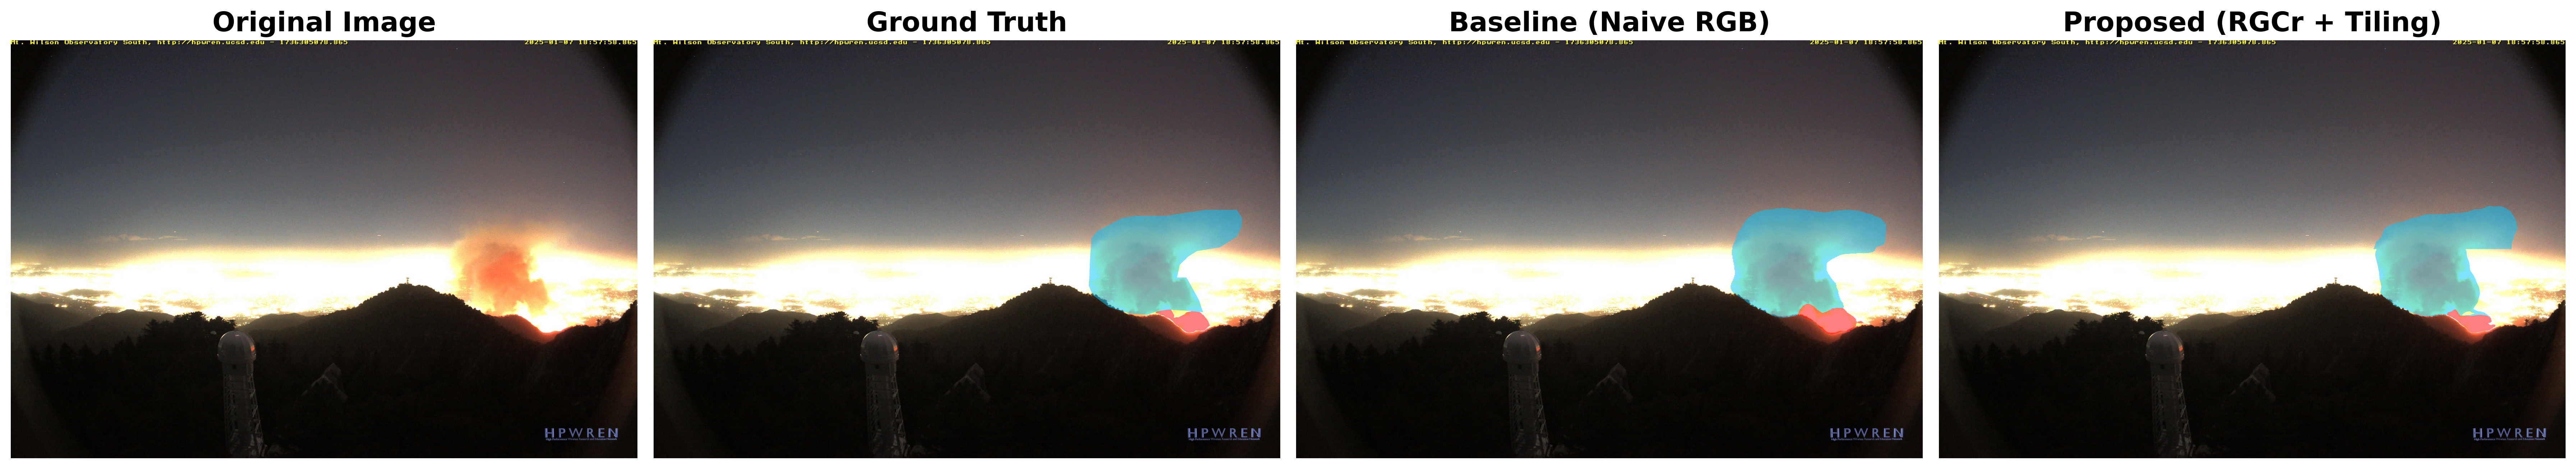
\includegraphics[width=\textwidth]{Figure_2_Qualitative_Comparison.png}}
\caption{Perbandingan kualitatif hasil segmentasi pada set pengujian FIgLib. Dari kiri ke kanan: (a) Gambar resolusi tinggi asli; (b) Anotasi Ground Truth yang menyoroti asap (cyan) dan api (merah); (c) Prediksi dari model Baseline Naif; (d) Prediksi dari Pipeline Usulan. Model baseline berhasil mendeteksi api namun memprediksi batasnya secara berlebihan, menghasilkan segmentasi yang sangat tidak presisi dan terlalu luas. Sebaliknya, combined loss dan pipeline data yang diusulkan memungkinkan arsitektur PIDNet-M untuk menggambarkan batas-batas fitur pembakaran minoritas dengan sangat rapat dan akurat.}
\label{fig:qualitative}
\end{figure*}

\section{Kesimpulan dan Pekerjaan Masa Depan}
Dalam makalah ini, kami membuktikan bahwa efisiensi arsitektur harus disandingkan dengan optimalisasi data dan loss yang agresif agar berhasil di lingkungan yang ekstrem. Kami menunjukkan bahwa arsitektur PIDNet-M standar gagal secara bencana pada kelas Api minoritas (mIoU 62,1\%) saat dihadapkan dengan ketidakseimbangan kelas 1:7. Dengan memperkenalkan Combined Loss Lovasz-Focal-Dice kustom, kami menyelamatkan performa kelas minoritas menjadi 79,9\%. Selain itu, dengan mengintegrasikan algoritme Balanced SAHI-style Tiling dan transformasi ruang warna RGCr, pipeline yang diusulkan berhasil meningkatkan Fire mIoU ke angka \textit{state-of-the-art} sebesar 81,14\%. Secara keseluruhan, metodologi kami memberikan peningkatan performa absolut sebesar lebih dari 19\% dibandingkan baseline standar. Hasil ini membuktikan secara definitif bahwa \textit{data-centric tuning} sama pentingnya dengan desain jaringan struktural untuk penerapan sistem pengawasan keselamatan hidup di dunia nyata.

\section*{Ketersediaan Kode}
Kode sumber, model pre-trained, dan pembagian dataset yang digunakan dalam studi ini tersedia di: \url{https://github.com/YourUsername/YourRepository}.

\begin{thebibliography}{00}
\bibitem{muhammad2023fire} I. Muhammad, F. Sthevanie, dan K. N. Ramadhani, ``Fire Detection using Combined Approach of HSV-based Harris Corner Region Extraction and Vision Transformer Classification,'' dalam \textit{2023 International Conference on Data Science and Its Applications (ICoDSA)}, IEEE, 2023, hal. 117-122.
\bibitem{pidnet} J. Xu, Z. Xiong, S. P. Bhattacharyya, ``PIDNet: A Real-time Semantic Segmentation Network Inspired by PID Controllers,'' dalam \textit{Proceedings of the IEEE/CVF Conference on Computer Vision and Pattern Recognition (CVPR)}, 2023, hal. 19529-19539.
\bibitem{sahi} F. C. Akyon, S. O. Altinuc, dan A. Temizel, ``Slicing Aided Hyper Inference and Fine-tuning for Small Object Detection,'' dalam \textit{2022 IEEE International Conference on Image Processing (ICIP)}, 2022, hal. 966-970.
\bibitem{focal} T. -Y. Lin, P. Goyal, R. Girshick, K. He, dan P. Dollár, ``Focal Loss for Dense Object Detection,'' dalam \textit{IEEE Transactions on Pattern Analysis and Machine Intelligence}, vol. 42, no. 2, hal. 318-327, Feb. 2020.
\bibitem{lovasz} M. Berman, A. Rannen Triki, dan M. B. Blaschko, ``The Lovász-Softmax loss: A tractable surrogate for the optimization of the intersection-over-union measure in neural networks,'' dalam \textit{Proceedings of the IEEE Conference on Computer Vision and Pattern Recognition (CVPR)}, 2018, hal. 4413-4421.
\bibitem{salehi2017tversky} S. S. M. Salehi, D. Erdogmus, dan A. Gholipour, ``Tversky loss function for image segmentation using 3D fully convolutional deep networks,'' dalam \textit{International Workshop on Machine Learning in Medical Imaging}, Springer, 2017, hal. 379-387.
\bibitem{he2009imbalanced} H. He dan E. A. Garcia, ``Learning from imbalanced data,'' dalam \textit{IEEE Transactions on Knowledge and Data Engineering}, vol. 21, no. 9, hal. 1263-1284, Sept. 2009.
\bibitem{buda2018systematic} M. Buda, A. Maki, dan M. A. Mazurowski, ``A systematic study of the class imbalance problem in convolutional neural networks,'' dalam \textit{Neural Networks}, vol. 106, hal. 249-259, 2018.
\bibitem{wu2019adaframe} Z. Wu, C. Shen, dan A. van den Hengel, ``AdaFrame: Adaptive Frame Selection for Fast Video Recognition,'' dalam \textit{Proceedings of the IEEE/CVF Conference on Computer Vision and Pattern Recognition (CVPR)}, 2019, hal. 1278-1287.
\bibitem{drummond2003c4} C. Drummond dan R. C. Holte, ``C4.5, class imbalance, and cost updating: an empirical study,'' dalam \textit{ICML Workshop on Learning from Imbalanced Datasets}, 2003.
\bibitem{govil2020preliminary} K. Govil, M. L. Welch, J. T. Epstein, dan J. K. MacAlpine, ``Preliminary results from a wildfire detection system using deep learning on remote camera images,'' dalam \textit{Remote Sensing}, vol. 12, no. 1, hal. 166, 2020.
\bibitem{nguyen2023smokeynet} T. Nguyen, J. H. Park, A. Mai, D. W. O'Brien, dan I. Altintas, ``SmokeyNet: Multimodal Wildland Fire Smoke Detection,'' dalam \textit{Remote Sensing}, vol. 15, no. 11, hal. 2883, 2023.
\end{thebibliography}

\end{document}
